\section{问题二模型建立与求解}

\subsection{问题二分析}

问题二在每日零时承诺整天购电量，但真实负载和光伏尚未知晓。计划量偏少时须支付五倍交易电价补足，偏多时已付费用不能收回。因而把一条均值预测直接代入问题一，未必能得到期望费用最低的采购量。储能同时参与价格套利和误差补偿，某时段的预测误差还会改变后续可用电量，必须按完整轨迹评估。

本问采用“因果预测、整日残差场景、共同采购计划、实际状态反馈”的方案\cite{abunima2022,marino2018,grover2018}。母模型预先关闭额外CVaR及备用，即$\lambda=0$、$\rho_t=0$，场景数保留此前最多28条历史轨迹。预测器和执行器在一月验证中按实际账单选择，风险偏好与场景压缩只做后续对照。本问的候选筛选在开发期未取得节费收益，因此最终仍采用母模型；滚动问题的筛选选型另见第三问。

\subsection{问题二模型建立}

\subsubsection{五倍补购费用为何导出80\%采购分位数}

先去掉储能和跨时段耦合，研究单时段基准。设$X$为实际净需求电量，$q\ge0$为计划采购，固定电价$p>0$，富余无残值，且$\mathbb E[X_+]<\infty$。概率和期望均以决策时已知信息为条件。期望费用为
\begin{equation}
 J_2(q)=pq+5p\,\mathbb E[(X-q)_+].
 \label{eq:mech_q2_cost}
\end{equation}
第一项是无论是否使用都要支付的计划费，第二项是计划不足时的补购费。记$F_X(x)=\Pr(X\le x)$、$F_X(x^-)=\Pr(X<x)$。$J_2$为凸函数，左右导数给出的次梯度为
\begin{equation}
 \partial J_2(q)=p[5F_X(q^-)-4,\ 5F_X(q)-4].
 \label{eq:mech_q2_subgradient}
\end{equation}
对于$q>0$的内点，最优解的充要条件是零属于其次梯度，即
\begin{equation}
 F_X(q^-)\le0.8\le F_X(q).
 \label{eq:mech_q2_quantile_condition}
\end{equation}
若分布在最优点连续，则$J_2'(q)=p-5p\Pr(X>q)=0$，化为$F_X(q)=0.8$；离散场景存在概率跳跃时，使用式\eqref{eq:mech_q2_quantile_condition}，不强求累积概率恰好等于0.8。若最优点位于$q=0$边界，则右导数非负要求$F_X(0)\ge0.8$。以下分位数$F_X^{-1}(\alpha)=\inf\{x:F_X(x)\ge\alpha\}$表示，可选取
\begin{equation}
 q_2^\star=\max\{0,F_X^{-1}(0.8)\}.
 \label{eq:mech_q2_quantile}
\end{equation}
平坦分布区间可能导致多个最优解，上式给出其中一个。

这说明采购高于均值可能只是最小化期望费用的结果，无须额外诉诸风险厌恶。80\%源于计划价格与五倍补购价格的比例；加入储能后还存在效率、功率、容量及跨时段机会价值，该阈值只作机制解释和简化基准，不能直接逐时套用，也不是后文备用误差分位数的理论依据。

\subsubsection{因果预测与决策导向选型}

问题二只使用附件1电价和附件2历史负载、光伏，不使用附件3发布预报。候选负载预测为前一周、最近2个或4个同星期日的同一时段均值，光伏预测为此前3、7或14个完整日的同一时段均值。以$X$表示负载，同星期预测写为
\begin{equation}
 \widehat X_{D,t}=\frac{1}{|\mathcal W_D|}\sum_{j\in\mathcal W_D}X_{j,t},\qquad
 \mathcal W_D=\{D-7i:i=1,\ldots,K\}\cap\{1,\ldots,D-1\}.
 \label{eq:weekday_forecast}
\end{equation}
光伏移动均值改用此前$K$个完整日。历史不足时利用已有样本，没有相应星期日则退回近7日均值，首日采用附件1固定先验。为其他问题生成的历史价格预测可使用同一形式；每个历史预测都只使用其日期以前的数据，不能把实际未来曲线作为预测。

文献\cite{elmachtoub2017spo}提出按预测引致的下游决策损失评价预测。本题借鉴这一思想，在固定相同场景和控制器的条件下比较候选预测器的实际结算费用，而不只按RMSE选择。未采用SPO或SPO+训练算法，也不引述其训练理论为本程序保证。

验证窗口为1月15--31日。同一问题的所有候选均从冻结旧版策略在1月15日的实际电量7081.8620 kWh开始，逐日因果运行，选择分数为计划费加紧急费，不含终端罚项。先固定28场景、无风险及备用的内层LP，比较负载方法，再固定选中的负载方法比较光伏；随后固定预测器比较贪心与内层LP。该分步搜索并未穷举预测和控制的全部组合。

% Generated by code/make_question_tables.py; do not edit values.
% Source: data/selection_v2.json; SHA256=f290084567f8b335dfbe7c042da7bf6863af20d3db001376f8bb5003dedd9aa7
\begin{table}[htbp]\centering\small
\caption{问题二预测器的一月实际费用验证}
\label{tab:q2-forecast-validation}
\begin{tabularx}{\linewidth}{LLLR}\toprule
比较步骤 & 负载预测 & 光伏预测 & 实际费用/元\\\midrule
负载比较 & 前一周 & 最近7日 & 933430.35\\
负载比较 & 同星期2日 & 最近7日 & 929216.46\\
负载比较 & 同星期4日 & 最近7日 & 930211.02\\
光伏比较 & 同星期2日 & 最近3日 & 928995.30\\
光伏比较 & 同星期2日 & 最近7日 & 929216.46\\
光伏比较 & 同星期2日 & 最近14日 & 932521.33\\
\bottomrule\end{tabularx}
\par\smallskip\parbox{\linewidth}{\footnotesize 此处固定内层LP及其余设置；相同配置复用同一次计算。随后单独比较执行器。费用不含终端目标项。}
\end{table}


由表\ref{tab:q2-forecast-validation}确定负载采用最近2个同星期日均值、光伏采用近3日均值。在这一预测组合下，贪心执行的一月费用917318.59元，内层LP为928995.30元，故主案选择贪心规则。两者一月验证末库存分别7155.31和6000.00 kWh，未强制相等，不能把费用比较表述为库存价值已经中和。

2月初态共同承接已冻结旧版1月实际末态8875.1909 kWh，不用一月底选出的新方法事后回写1月。验证轨迹用于选型，旧版一月运行轨迹用于提供共同前缀，两者不能混淆。2月以后预测器类型、实时控制器及母模型设置固定，实际SOC连续传递；候选筛选的适用问题与启用时点依据2--12月开发性回测确定。因此，本文报告开发期闭环评价，不称为完全未见数据上的独立测试。

\subsubsection{整日历史残差与场景构造}

在日期$D$的零时，取此前至多28个完整日组成$\mathcal H_D$。历史日$j$在时段$t$的净负荷残差为
\begin{equation}
 \epsilon^n_{j,t}=
 \big[(L_{j,t}-R_{j,t})-(\widehat L_{j,t}-\widehat R_{j,t})\big]\Delta t,
 \qquad j<D.
 \label{eq:residual}
\end{equation}
每个历史日保留为完整144段轨迹，当前场景由
\begin{equation}
 n_{t,s}=\widehat n_t+\epsilon^n_{j_s,t},\qquad
 \pi_s=1/|\mathcal H_D|,\qquad \sum_s\pi_s=1
 \label{eq:q2_empirical_scenarios}
\end{equation}
给出。这样保留连续几小时共同偏高或偏低的误差，避免独立逐点抽样破坏时间关联。历史充足后排除采用固定先验的1月1日，主填报期均保留28条历史日轨迹。经验分布只代表有限窗口内出现过的误差，不等于真实未来分布。

场景缩减对照取最多12个代表日。对历史误差按整个残差块的总体标准差归一，计算轨迹间欧氏距离；先选总距离最小的代表，再逐次加入离已有代表最远的轨迹，随后交替分配样本与更新簇内medoid，至代表不变或达到8轮。每个代表仍是实际历史日，概率为所属簇频率。压缩改变场景及权重，其经济效果另行验证，不视为不影响结果的纯计算简化。

\subsubsection{受限两阶段采购模型}

日前第一阶段选择所有场景共享的计划$g_t$及参考$c_t,d_t,e_{t+1}$；补救阶段只允许紧急购电$h_{t,s}$随场景变化：
\begin{equation}
 g_t+d_t+h_{t,s}-c_t\ge n_{t,s},\qquad h_{t,s}\ge0.
 \label{eq:scenario_balance}
\end{equation}
同一组参考充放电须在所有场景下配合相应紧急补购满足净需求。以
$Q_s=\sum_t5p_th_{t,s}$表示一条完整场景的紧急费用，主目标为
\begin{equation}
 \min\left\{\sum_tp_tg_t+\sum_s\pi_sQ_s+
 \beta_T|e_{144}-6000|\right\},\qquad
 \beta_T=b_T\operatorname{median}_{t}p_t,\quad b_T=1.
 \label{eq:q2_objective}
\end{equation}
第一项是零时承诺的计划费，第二项按场景概率计算期望紧急费，二者体现本题的非对称结算。第三项是有限时域库存价值的软近似，抑制单纯为缩短本日账单而在日末过度放电的倾向，不计入实际账单，也不强制每天恢复6000 kWh。绝对值通过正负偏差变量线性化。容量、功率和状态方程沿用式\eqref{eq:soc}、\eqref{eq:limits}，初态使用当日实际SOC，购电非负。

该模型是受限两阶段随机规划，而非完全多阶段策略。共享储能参考避免对每个场景独立优化整天、提前知道未来情况；但实际控制会利用逐时观测调整储能，参考紧急费仍可能不同于真实执行费用。本文分别保留参考和实际轨迹，不把外层$c_t,d_t$直接作为附件5的实际充放电量。

\subsubsection{贪心执行器及状态连续性}

零时购电计划一经确定，本问全天令$a_t=g_t$。当期可观测的有效采购$a_t$、净需求$n_t$和储电量$e_t$决定实际动作。若$a_t\ge n_t$：
\begin{equation}
 c_t^{\rm act}=\min\{a_t-n_t,U,(E_{\max}-e_t)/\eta_c\},\quad
 d_t^{\rm act}=h_t=0,\quad w_t=a_t-n_t-c_t^{\rm act}.
 \label{eq:execute_charge}
\end{equation}
若$a_t<n_t$：
\begin{equation}
 d_t^{\rm act}=\min\{n_t-a_t,U,\eta_d(e_t-E_{\min})\},\quad
 c_t^{\rm act}=w_t=0,\quad h_t=n_t-a_t-d_t^{\rm act}.
 \label{eq:execute_discharge}
\end{equation}
然后按式\eqref{eq:soc}更新状态。此规则优先以常规富余充电、以当前电量补缺，不足部分紧急购买，不用紧急电量主动充电。充放电互斥、容量和功率约束逐步得到满足，外网补购使实际负载得到保障。

日际满足$e_{D+1,0}=e_{D,144}$，不每日重置。执行器不直接读取当前或未来价格、参考SOC和参考备用，因此其与场景规划的差异仍然存在。后续问题会用固定合同回放和内层LP专门检查这种差异；贪心被一月账单选中，不代表已经证明它是所有因果控制策略中的最优解。

\subsubsection{风险与备用的可选扩展}

经济主案取$\lambda=\rho_t=0$。为了识别额外保守程度的影响，对照在式\eqref{eq:q2_objective}加入$\lambda\operatorname{CVaR}_{0.90}(Q)$。其中$Q$只含紧急费用，不是全天总账单；按照文献\cite{rockafellar2000}写为
\begin{equation}
 \operatorname{CVaR}_{\alpha}(Q)=
 \min_z\left\{z+\frac{1}{1-\alpha}\sum_s\pi_sv_s\right\},\quad
 v_s\ge Q_s-z,\quad v_s\ge0,\quad\alpha=0.90.
 \label{eq:cvar}
\end{equation}
自适应权重根据近期残差总体标准差设定：
\begin{equation}
 \lambda=0.10\min\{3,r/0.20\},\qquad
 r=\frac{\operatorname{mean}_t\operatorname{sd}_j(\epsilon^n_{j,t})}
 {\max\{\operatorname{mean}_t|\widehat n_t|,50\}}.
 \label{eq:risk_weight}
\end{equation}
标准差分母取历史样本日数，50 kWh防止净需求接近零时比值失稳。固定风险权重则取一月自适应序列均值0.10368，不能用2--12月数据重新匹配。

参考备用沿同一历史日累加未来至多六段误差，以外侧累计缺口换算为内部库存：
\begin{align}
 \rho_t^{\rm raw}
 &=k_\rho\min\left\{2400,
 \frac{\left[q_{0.8}\left(\sum_{k=t+1}^{\min(t+6,143)}
             \epsilon^n_{j,k}\right)\right]_+}{\eta_d}\right\},
 \label{eq:reserve}\\
 \rho_t&=\min\{\rho_t^{\rm raw},
 [e_\tau-E_{\min}+\eta_cU(t-\tau+1)]_+\},\qquad
 e_{t+1}\ge E_{\min}+\rho_t.
 \label{eq:reachable_reserve}
\end{align}
本问$\tau=0$，后续滚动问题可取其他发布时点。分位数按排序样本间线性插值，空和为零；先在2400 kWh截断，再乘无量纲$k_\rho$，故缩放后的上限为$2400k_\rho$。最后按当前电量及最大充电速度做可达截断。该处理与先缩放再重新截到2400不同，复现时须保持顺序。

动态备用对照取$k_\rho=1$；固定备用取一月可达截断前动态备用均值208.67 kWh，日末置零，再作相同可达截断。一月匹配按每次外层更新实际覆盖的时段计数。备用仅限制外层参考轨迹，实际执行器可为当期负载消耗它，物理下限仍为1200 kWh，不能解释成保证80\%供电可靠性的硬约束。终端系数$\beta_T$单位为元/kWh，备用系数$k_\rho$无量纲，二者分开记号。

\subsection{问题二求解}

\subsubsection{逐日求解与评价口径}

每天零时先读取之前已完成的负载及光伏，更新冻结类型的预测器，再按式\eqref{eq:residual}构造28条场景；以当前实际SOC为初态求解外层LP，保存整日原计划和参考储能。随后每10分钟只揭示当前实际负载、光伏，按式\eqref{eq:execute_charge}或\eqref{eq:execute_discharge}执行，将本段充放电、紧急量及末态写入实际数组。当天结束后按
\begin{equation}
 C_D=\sum_{t=0}^{143}p_tg_{D,t}+\sum_{t=0}^{143}5p_th_{D,t}
 \label{eq:q2_actual_bill}
\end{equation}
重新结算，并把末态传至下一日。优化器的CVaR、终端项及数值破同解项都不进入该账单。

正式评价范围为2025年2月1日至12月31日334天、每天144段。除核对费用可加性外，还检查实际电量平衡、SOC递推、充放电互斥、上下界、日际连续性以及全天$a_t=g_t$。指定日表、日汇总和附件5均从同一执行数组生成，原模板表头和列序保持不变。

预测的RMSE及MAE只描述所选方法，不参与回测期再选型。表\ref{tab:q2-prediction-errors}给出实际误差，说明低成本采购仍建立在有误差的预测之上。
% Generated by code/make_question_tables.py; do not edit values.
% Source: data/selection_v2.json; SHA256=f290084567f8b335dfbe7c042da7bf6863af20d3db001376f8bb5003dedd9aa7
% Source: data/prepared_v2_q2.npz; SHA256=0322336272736ef1956aefa31f183bf42740abd1797e8d0d290fc61a700158fa
\begin{table}[htbp]\centering\small
\caption{问题二已选预测器的误差，单位为kW}
\label{tab:q2-prediction-errors}
\begin{tabularx}{\linewidth}{LRRRR}\toprule
变量 & 一月MAE & 一月RMSE & 评价期MAE & 评价期RMSE\\\midrule
负载 & 122.51 & 152.09 & 171.91 & 240.54\\
光伏 & 100.38 & 214.94 & 154.46 & 313.48\\
\bottomrule\end{tabularx}
\par\smallskip\parbox{\linewidth}{\footnotesize 一月指标取1月15--31日，评价期取2--12月。类型按一月结算费用选择，表中误差不用于重选。}
\end{table}


\subsubsection{总体结果与基础方案比较}

计划费用13507968.43元、紧急费用504839.24元，总费用14012807.66元；各分项分别四舍五入时可能与总数相差0.01元，汇总统一从原精度计算。全天计划购电22047537.09 kWh，紧急购电85017.69 kWh，后者涉及113天、617个10分钟时段。年末库存6240.32 kWh，低于共同期初8875.19 kWh，因此比较账单时须同时看库存，不称其为库存中性节费。

\begin{table}[htbp]\centering\small
\caption{问题2在相同预测与初态下的基础对照}
\label{tab:v2_baselines}
\begin{tabularx}{\linewidth}{LRRRR}\toprule
策略 & 总费/万元 & 紧急量/kWh & 日费CVaR95/元 & 末库存/kWh\\\midrule
无储能场景采购 & 1854.80 & 242340.86 & 80425.37 & 8875.19\\
点预测采购 & 1529.08 & 505585.75 & 100557.90 & 5845.40\\
场景期望费用（主案） & 1401.28 & 85017.69 & 70731.74 & 6240.32\\
\bottomrule\end{tabularx}
\par\smallskip\parbox{\linewidth}{\footnotesize 本表基于未启用候选筛选的母模型，各组保留原实验配置及数值，覆盖相同334天并连续推进状态；不作为最终筛选算法的同条件消融。}
\end{table}


表\ref{tab:v2_baselines}的三组使用相同预测和期初库存。点预测采购仅把预测曲线输入调度器，无储能场景采购则禁用充放电，其他经济设置保持一致。点预测费用15290840.75元，主案节省1278033.08元，即8.36\%；相较无储能场景采购18548033.07元，主案费用降低24.45\%。主要证据支持历史场景对非对称补购代价的处理及储能跨时段转移，而不是必须加入CVaR。紧急购电已支付高额代价但补足了负载，其发生不表示实际已经失供电。

图\ref{fig:q2-calendar-heatmap}按日期和物理时段联合展示紧急购电与时段末SOC，可定位缺口在一天中的位置，以及是否伴随库存接近下限。零紧急量留浅灰，正值采用幂次色阶突出稀疏小额事件，色条仍标原始kWh；库存使用独立的固定上下界色标。不能仅凭两个面板的颜色深浅把补购量和库存直接作等量比较。
\begin{figure}[htbp]\centering
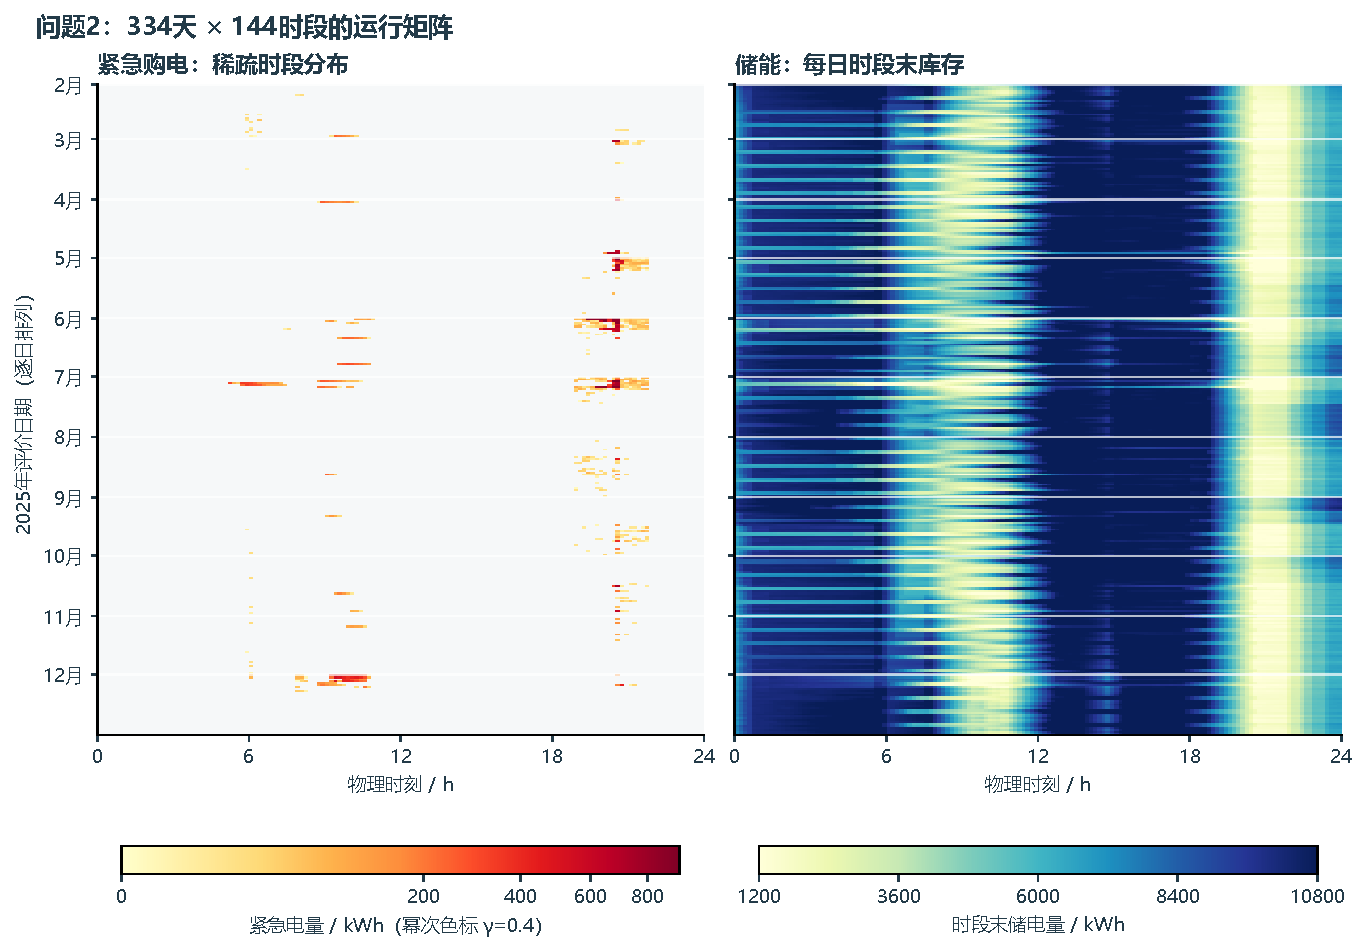
\includegraphics[width=0.97\linewidth]{figures/results/q2_calendar_heatmap.pdf}
\caption{问题二334个日期与144个物理时段的紧急量和时段末SOC；紧急量正值采用$\gamma=0.4$幂次色标，颜色数值仍以kWh标示}
\label{fig:q2-calendar-heatmap}
\end{figure}

基于执行规则回放的候选筛选在本问得到费用14035379.65元，比母模型增加22571.98元，即0.161\%，紧急量也增至138015.18 kWh。因此本问不启用该模块。它在滚动采购中的适用性及筛选时点比较见第三问，不能由滚动组节费推断日前采购同样受益。

\subsubsection{题目指定日期与完整策略填报}

\begin{table}[htbp]\centering\small
\caption{问题2指定日期购电结果（沿用题目表1布局，电量单位：kWh）}
\label{tab:q2-purchase}
\par\smallskip\textbf{2025-03-20}\par\smallskip
\begin{tabularx}{\linewidth}{lRlRlR}
\toprule
时间段 & 购电量 & 时间段 & 购电量 & 时间段 & 购电量\\
\midrule
10:00--10:10 & 0.00 & 12:00--12:10 & 564.20 & 14:00--14:10 & 0.00\\
16:00--16:10 & 490.32 & 18:00--18:10 & 704.86 & 20:00--20:10 & 0.00\\
\midrule
全天购电量 & 67796.64 & \multicolumn{2}{c}{全天购电费（元）} & \multicolumn{2}{r}{41219.41}\\
\bottomrule
\end{tabularx}
\par\smallskip\textbf{2025-06-21}\par\smallskip
\begin{tabularx}{\linewidth}{lRlRlR}
\toprule
时间段 & 购电量 & 时间段 & 购电量 & 时间段 & 购电量\\
\midrule
10:00--10:10 & 0.00 & 12:00--12:10 & 0.00 & 14:00--14:10 & 0.00\\
16:00--16:10 & 296.43 & 18:00--18:10 & 275.52 & 20:00--20:10 & 0.00\\
\midrule
全天购电量 & 40036.30 & \multicolumn{2}{c}{全天购电费（元）} & \multicolumn{2}{r}{23986.38}\\
\bottomrule
\end{tabularx}
\par\smallskip\textbf{2025-09-23}\par\smallskip
\begin{tabularx}{\linewidth}{lRlRlR}
\toprule
时间段 & 购电量 & 时间段 & 购电量 & 时间段 & 购电量\\
\midrule
10:00--10:10 & 0.00 & 12:00--12:10 & 475.29 & 14:00--14:10 & 0.00\\
16:00--16:10 & 537.29 & 18:00--18:10 & 789.93 & 20:00--20:10 & 0.00\\
\midrule
全天购电量 & 69576.50 & \multicolumn{2}{c}{全天购电费（元）} & \multicolumn{2}{r}{46384.26}\\
\bottomrule
\end{tabularx}
\par\smallskip\textbf{2025-12-21}\par\smallskip
\begin{tabularx}{\linewidth}{lRlRlR}
\toprule
时间段 & 购电量 & 时间段 & 购电量 & 时间段 & 购电量\\
\midrule
10:00--10:10 & 0.00 & 12:00--12:10 & 970.92 & 14:00--14:10 & 0.00\\
16:00--16:10 & 851.12 & 18:00--18:10 & 744.23 & 20:00--20:10 & 0.00\\
\midrule
全天购电量 & 101008.53 & \multicolumn{2}{c}{全天购电费（元）} & \multicolumn{2}{r}{65454.44}\\
\bottomrule
\end{tabularx}
\par\smallskip\parbox{\linewidth}{\footnotesize 注：问题2与4-2列示计划购电量；问题3与4-3列示最终生效的调整后常规购电量。全天购电量不含紧急购电，全天购电费含计划、调整与紧急费用。}
\end{table}

\begin{table}[htbp]\centering\small
\caption{问题2指定日期储能结果（沿用题目表2布局，单位：kWh）}
\label{tab:q2-battery}
\par\smallskip\textbf{2025-03-20}\par\smallskip
\begin{tabularx}{\linewidth}{lRRlRR}
\toprule
时间段 & 充电量 & 放电量 & 时间段 & 充电量 & 放电量\\
\midrule
00:00--04:00 & 3924.13 & 181.53 & 04:00--08:00 & 1015.09 & 5240.21\\
08:00--12:00 & 6123.03 & 2777.38 & 12:00--16:00 & 3923.99 & 420.71\\
16:00--20:00 & 268.54 & 5719.49 & 20:00--24:00 & 5703.85 & 2960.43\\
\midrule
0:00储电量 & \multicolumn{2}{r}{6705.54} & 24:00储电量 & \multicolumn{2}{r}{6346.37}\\
\bottomrule
\end{tabularx}
\par\smallskip\textbf{2025-06-21}\par\smallskip
\begin{tabularx}{\linewidth}{lRRlRR}
\toprule
时间段 & 充电量 & 放电量 & 时间段 & 充电量 & 放电量\\
\midrule
00:00--04:00 & 1394.50 & 465.11 & 04:00--08:00 & 460.19 & 4390.39\\
08:00--12:00 & 6534.90 & 0.00 & 12:00--16:00 & 0.00 & 0.00\\
16:00--20:00 & 156.59 & 4882.20 & 20:00--24:00 & 6792.80 & 2485.90\\
\midrule
0:00储电量 & \multicolumn{2}{r}{8644.37} & 24:00储电量 & \multicolumn{2}{r}{8867.68}\\
\bottomrule
\end{tabularx}
\par\smallskip\textbf{2025-09-23}\par\smallskip
\begin{tabularx}{\linewidth}{lRRlRR}
\toprule
时间段 & 充电量 & 放电量 & 时间段 & 充电量 & 放电量\\
\midrule
00:00--04:00 & 4692.99 & 53.14 & 04:00--08:00 & 916.24 & 5893.48\\
08:00--12:00 & 5977.49 & 1896.62 & 12:00--16:00 & 3708.39 & 625.98\\
16:00--20:00 & 151.78 & 5739.35 & 20:00--24:00 & 5609.40 & 2640.89\\
\midrule
0:00储电量 & \multicolumn{2}{r}{6006.02} & 24:00储电量 & \multicolumn{2}{r}{6235.06}\\
\bottomrule
\end{tabularx}
\par\smallskip\textbf{2025-12-21}\par\smallskip
\begin{tabularx}{\linewidth}{lRRlRR}
\toprule
时间段 & 充电量 & 放电量 & 时间段 & 充电量 & 放电量\\
\midrule
00:00--04:00 & 4499.79 & 40.16 & 04:00--08:00 & 762.27 & 1359.20\\
08:00--12:00 & 5913.75 & 6490.57 & 12:00--16:00 & 5645.48 & 2130.65\\
16:00--20:00 & 0.00 & 5526.27 & 20:00--24:00 & 5771.81 & 2842.53\\
\midrule
0:00储电量 & \multicolumn{2}{r}{6794.81} & 24:00储电量 & \multicolumn{2}{r}{6695.97}\\
\bottomrule
\end{tabularx}
\end{table}

\begin{table}[htbp]\centering\small
\caption{问题2指定日期紧急购电（题目表3布局，单位：kWh）}
\label{tab:q2-emergency}
\setlength{\tabcolsep}{3pt}
\begin{tabularx}{\linewidth}{lRlRlRlR}\toprule
\multicolumn{2}{c}{2025-03-20} & \multicolumn{2}{c}{2025-06-21} & \multicolumn{2}{c}{2025-09-23} & \multicolumn{2}{c}{2025-12-21}\\
时间段 & 购电量 & 时间段 & 购电量 & 时间段 & 购电量 & 时间段 & 购电量\\\midrule
无 & 0.00 & 无 & 0.00 & 20:20--20:40 & 388.40 & 无 & 0.00\\
 &   &  &   & 20:50--21:10 & 90.05 &  &  \\
 &   &  &   & 21:20--21:50 & 34.20 &  &  \\
\midrule
合计 & 0.00 & 合计 & 0.00 & 合计 & 512.64 & 合计 & 0.00\\
\bottomrule\end{tabularx}\end{table}

四个指定日中，9月23日存在三段紧急购电，合计512.64 kWh，其余三个指定日为零。其常规计划费用43098.28元，紧急费用3285.98元，全天实际费用46384.26元；不能把全天费用只写成计划量乘价格。相邻正值时段才合并为同一紧急区间，间隔含零时保持分段。

表\ref{tab:q2-purchase}的指定时段及全天购电量均指零时计划，不含紧急量；后者单列于表\ref{tab:q2-emergency}。表\ref{tab:q2-battery}填写实际动作，各四小时块内充放电均可能为正，但每个10分钟段仍互斥。完整计划保存在\texttt{result2.xlsx}，日费用分解可由同源结果数据核对。
\FloatBarrier

\subsubsection{风险、备用及其联合作用}

\begin{table}[htbp]\centering\small
\caption{问题2风险与备用的完整对照}
\label{tab:v2_risk_modules}
\begin{tabularx}{\linewidth}{LRRRR}\toprule
策略 & 总费/万元 & 紧急量/kWh & 日费CVaR95/元 & 末库存/kWh\\\midrule
期望费用 & 1401.28 & 85017.69 & 70731.74 & 6240.32\\
固定风险 & 1411.84 & 56316.17 & 69028.62 & 6318.65\\
自适应风险 & 1405.41 & 66920.81 & 69476.71 & 6255.33\\
固定备用 & 1401.09 & 74987.90 & 70409.51 & 6240.32\\
动态备用 & 1402.30 & 76168.28 & 70299.39 & 6245.11\\
固定风险+备用 & 1413.36 & 49102.47 & 68862.93 & 6318.65\\
自适应风险+备用 & 1406.93 & 59081.98 & 69070.96 & 6260.12\\
自适应联合，12场景 & 1404.26 & 75336.25 & 70065.84 & 6289.57\\
\bottomrule\end{tabularx}
\par\smallskip\parbox{\linewidth}{\footnotesize 本表基于未启用候选筛选的母模型，各组保留原实验配置及数值，覆盖相同334天并连续推进状态；不作为最终筛选算法的同条件消融。}
\end{table}

\begin{table}[htbp]\centering\small
\caption{固定与自适应策略在评价期实现的平均保守程度}
\label{tab:v2_conservatism}
\begin{tabularx}{\linewidth}{LRR}\toprule
策略 & 平均风险权重 & 平均参考备用/kWh\\\midrule
固定风险 & 0.10368 & 0.00\\
自适应风险 & 0.05506 & 0.00\\
固定备用 & 0.00000 & 207.22\\
动态备用 & 0.00000 & 244.39\\
固定联合 & 0.10368 & 207.22\\
自适应联合 & 0.05506 & 244.39\\
\bottomrule\end{tabularx}
\par\smallskip\parbox{\linewidth}{\footnotesize 固定参数由一月动态序列的均值匹配；由于季节与误差分布变化，评价期均值不保证相等，不用评价期重新匹配。}
\end{table}

与主案相比，仅固定风险增加105631.25元，仅自适应风险增加41280.51元，紧急量分别降至56316.17和66920.81 kWh。固定备用单独使用节省1891.73元，动态备用单独使用增加10152.11元，说明备用的经济效果取决于其形状和时段作用。联合自适应策略增加56524.93元，紧急量降至59081.98 kWh。紧急费用CVaR的优化目标和表中日总费用CVaR95不是同一个损失对象，不据其中一项下降推断另一项必然下降。

固定参数虽由一月均值匹配，评价期固定和自适应的平均风险权重分别为0.103681与0.055059，参考备用均值分别为207.22与244.39 kWh，并未保持相同。因此两类方法之间的差异同时包含保守程度变化，不能全部归结为自适应对高风险时段识别得更准确。

以$C_{\rm joint}-C_{\rm risk}-C_{\rm reserve}+C_{\rm expectation}$描述联合作用，固定和自适应两组分别为17088.03元和5092.30元，均为正。这意味着本回测中联合费用高于两项单独费用变化的简单相加，但不是独立因果效应估计，也不是普遍的重复保守定理。

\begin{figure}[htbp]\centering
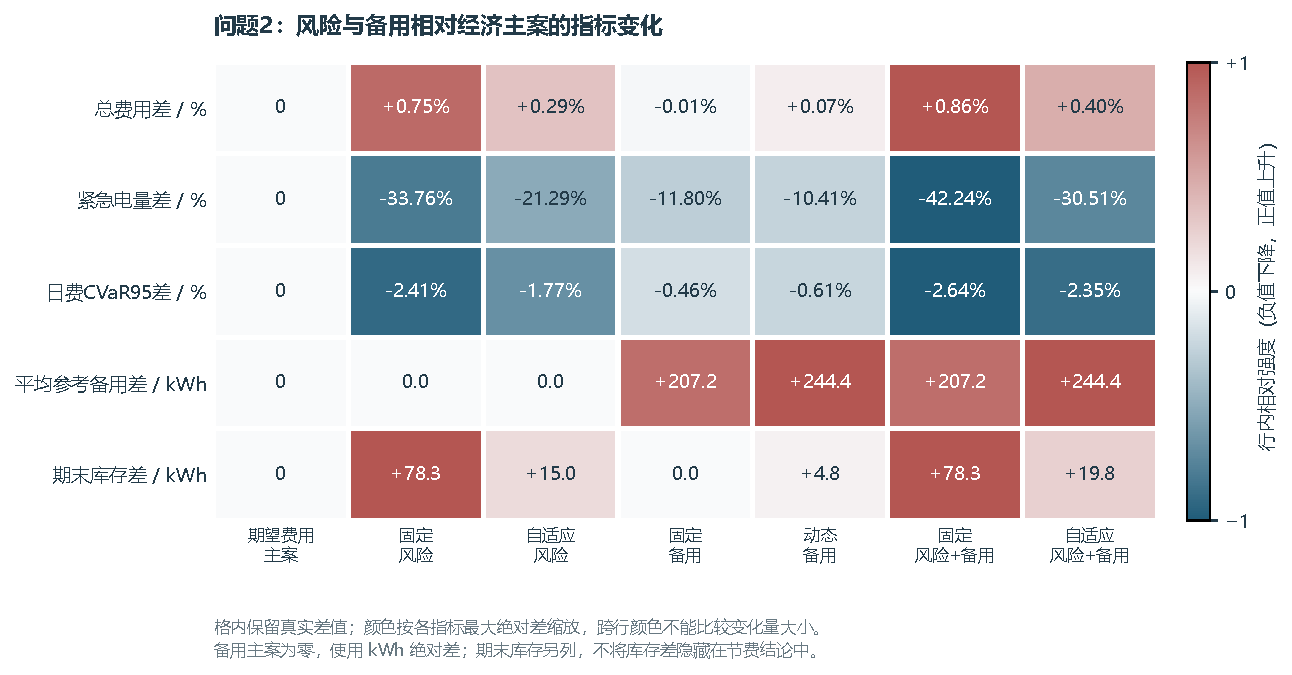
\includegraphics[width=0.95\linewidth]{figures/results/q2_risk_heatmap.pdf}
\caption{七种风险与备用设置相对主案的指标差异；前三行标注百分比，备用和末库存标注kWh差值，颜色仅在同一指标行内比较}
\label{fig:q2-risk-heatmap}
\end{figure}

图\ref{fig:q2-risk-heatmap}与完整对照表共同展示，紧急购电减少往往伴随额外常规承诺。费用、紧急量和日费CVaR95使用相对主案百分比变化；参考备用的主案值为零，故与末库存一样报告kWh差值。配色按各指标行的最大绝对变化归一，不跨行比较色深，也不将红色一律解释为不利。固定备用在评价期较便宜，也不据此替换预先冻结的主案。风险扩展回答的是为减少特定补购需求愿意支付多少费用，而非赛题额外规定了必须达到的安全阈值。

\subsubsection{28轨迹保留与12代表日压缩}

% Generated by code/make_question_tables.py; do not edit values.
% Source: data/experiments_v2.json; SHA256=e231ea14b234bd4593ec19c5f913ce028ed3b15ee677b4b58eafc7d3a658f29a
\begin{table}[htbp]\centering\small
\caption{问题二完整场景与压缩场景的同条件比较}
\label{tab:v2_scenarios}
\label{tab:v2_solve_times}
\begin{tabularx}{\linewidth}{LRRRR}\toprule
场景数 & 总费/万元 & 紧急量/kWh & 日费CVaR95/元 & 秒/日\\\midrule
28 & 1401.28 & 85017.69 & 70731.74 & 0.0521\\
12 & 1400.63 & 105407.24 & 72139.66 & 0.0276\\
\bottomrule\end{tabularx}
\par\smallskip\parbox{\linewidth}{\footnotesize 相同334天、预测、执行器及期初库存；末库存分别为6240.32和6257.26 kWh。时间包含预测、求解和执行，在本机并行条件下仅反映工程量级。}
\end{table}


经济目标下12场景比28场景少付6465.72元，却多购20389.55 kWh紧急电量，日费用CVaR95也更高。风险与备用联合开启时，12场景总费用14042623.21元、紧急量75336.25 kWh；28场景为14069332.59元、59081.98 kWh。压缩既改变期望费用，也会改变尾部及紧急需求，不能凭单一总费用接近就判断尾部已被保留。

28个等权历史日的10\%尾部仅有2.8条轨迹的概率质量，风险估计本来就受样本量限制；压缩后还可能集中到少数代表日。主案预定保留28条，排除额外压缩影响，求解耗时仍适合本题规模。该选择并不保证本年度实际账单最小，也不消除28日历史窗口有限性的限制。

为核对缩减程序的数值过程，另外记录334个日期窗口的实际medoid迭代。令标准化历史轨迹为$x_j$，第$m$轮代表集合为$\mathcal M^{(m)}$，压缩距离目标为
\begin{equation}
 J_m=\frac{1}{|\mathcal H_D|}\sum_{j\in\mathcal H_D}
       \min_{\ell\in\mathcal M^{(m)}}\|x_j-x_\ell\|_2.
 \label{eq:q2_compression_objective}
\end{equation}
图\ref{fig:q2-scenario-convergence}对每个窗口用其初值归一为$J_m/J_0$，再显示跨窗口中位数和P10--P90区间。334个窗口均达到代表稳定，迭代次数中位数2、最大5，最终相对目标中位数0.9816002。代表和权重已逐窗口与原缩减函数输出核对。

\begin{figure}[htbp]\centering
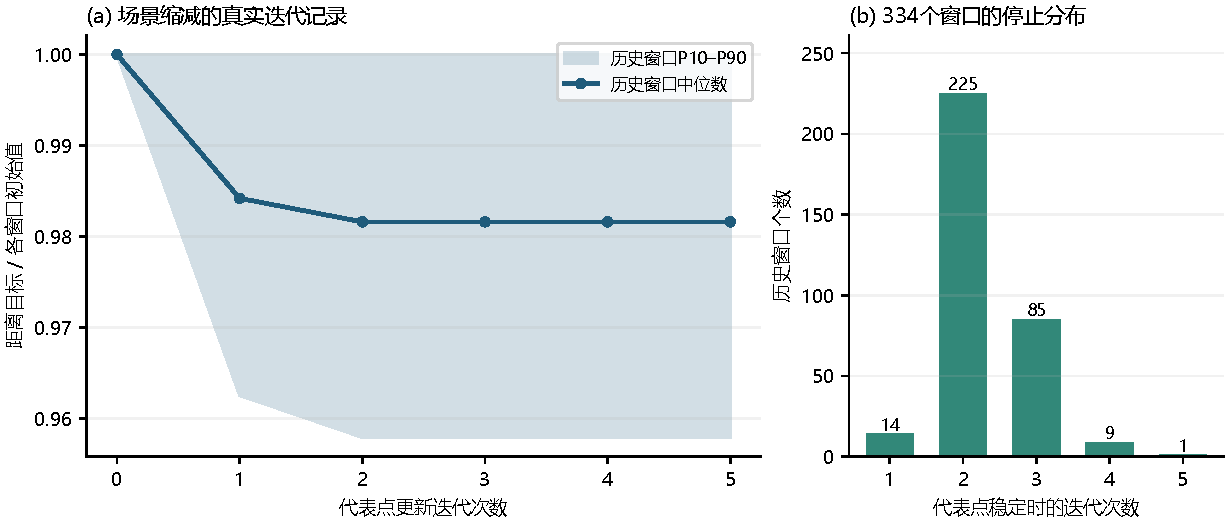
\includegraphics[width=0.93\linewidth]{figures/results/q2_scenario_convergence.pdf}
\caption{12代表日压缩距离目标的实际迭代；曲线为334窗口归一目标中位数，阴影为逐轮P10--P90}
\label{fig:q2-scenario-convergence}
\end{figure}

停止后的窗口只重复终值以对齐横轴，图中分位区间描述不同窗口之间的离散程度，不是置信带。此图证明的是历史轨迹几何压缩过程按预定准则稳定，并非LP求解收敛、经济费用下降或尾部风险保持；经济结论仍由表\ref{tab:v2_scenarios}及实际执行账单决定。
\FloatBarrier
